\chapter{Cloud Computing} \label{CloudComputingAnnexe}

  \section{Définition}
  Il existe autant de réponse à « Qu’est-ce que le Cloud Comptine ? » que de distribution linux. J’ai pour ma part décider de baser mon analyse sur la définition fournit par NIST (National Institut of Standards and Technology):\\

  \begin{quotation}
    \emph{« Cloud Computing is a model for enabling ubiquitous, convenient,on-demand network access to a shared pool of configurable Computing resources (e.g., networks, servers, storage, applications, and services) that can be rapidly provisioned and released with minimal management effort or service provider interaction. This Cloud model is composed of five essential characteristics, three service models, and four deployment models. »}
  \end{quotation}

  \begin{quotation}
    \emph{« Le Cloud Computing est un modèle qui permet un accès omniprésent, pratique et à la demande à un réseau partagé et à un ensemble de ressources informatiques configurables (comme par exemple : des réseaux, des serveurs, du stockage, des applications et des services) qui peuvent être provisionnées et libérées avec un minimum d’administration. »}\\
  \end{quotation}

  Pour simplifier, le Cloud Computing est la dématérialisation de l’informatique. C’est le fait de déporter toutes les opérations normalement effectuées sur nos ordinateurs sur des ordinateurs distants, autrement dit sur internet. L’ensemble de ses serveurs constituent le Cloud (Voir Figure \ref{Cloud Computing}).

  \begin{figure}
    \begin{center}
      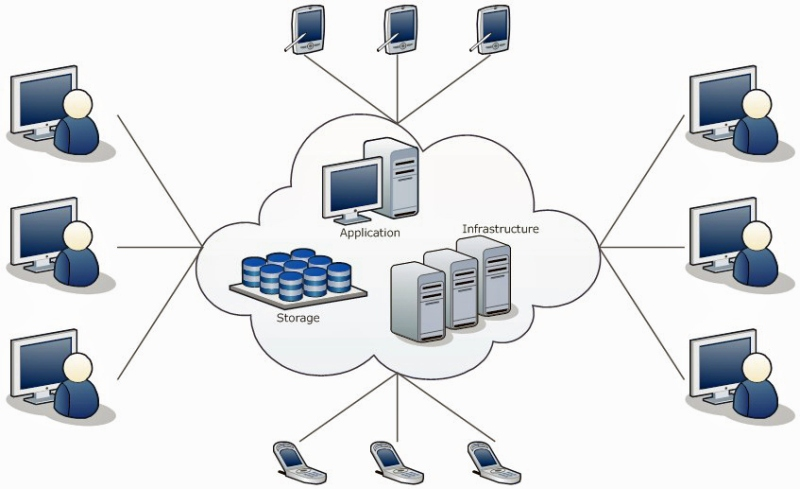
\includegraphics[scale=0.3]{images/CloudComputing.png}
    \end{center}
    \caption{Schématisation du Cloud Computing}
    \label{Cloud Computing}
  \end{figure}

  \subsection{Un service à la demande et une flexibilité des ressources.}
  Avec les applications Cloud, nous adaptons le flux de données à l'évolution de nos besoins: nous ne payons que pour ce que nous consommons. Et nous n'avons plus à nous soucier de manquer de capacité.

  \subsection{Accès universel par le réseau}
  Le terme de nuage représente bien le concept. Imaginons que nos ordinateurs nous suivent partout, que nous puissions y accéder n’importe où, n’importe quand depuis n’importe quel terminal. Imaginons un accès universel aux ressources stockés sur nos ordinateurs.

  \subsection{Une mise en commun des ressources}
  L'application de correctifs, la mise à niveau et le test d'applications peuvent occuper nos équipes informatique s plusieurs jours par mois. Grâce aux applications Cloud, cette problématique disparaît.\\

  Cependant ce n’est pas si simple que cela. Il existe trois types de Cloud: le Cloud public (loué par des prestataires), le Cloud privé (créer et gérer par notre entreprise) et le Cloud hybride (un mélange des deux précédents).

  \section{Le Cloud public}
  Le Cloud public appartient à des prestataires de service qui louent l’utilisation de leurs serveurs en facturant leur utilisation à la demande. Nous payons le flux de données échangé. Il dispose principalement de quatre modèles qui correspondent à des besoins bien distincts: le IAAS, le PASS, le SAAS et le STAAT.

    \subsection{Le Cloud IAAS ou Infrastructure As A Service (infrastructure en tant que service)}
    Le IAAS correspond à une infrastructure informatique (serveurs, réseaux, stockage) hébergé chez le prestataire de service. Nous n’avons pas besoin d’acheter le matériel nécessaire à notre infrastructure, nous nous contentons de la louer mais la gérons comme bon nous semble. Nous installons les serveurs que nous souhaitons utiliser et nous gérons l’ensemble des OS installés sur ces derniers. IAAS est utile si l’on désire créer ses propres plateformes pour ensuite y déployer des applications comme sur des serveurs locaux.

    \subsection{Le Cloud PAAS ou Plateform As A Service (plateforme en tant que service)}
    Le PAAS constitue l’utilisation par le biais d’internet de plateformes sur lesquelles nous pouvons déployer nos propres applications. C’est le niveau d’exécution des logiciels. Nous louons une plateforme, c’est à dire une machine avec un OS, le tout prêt à l’emploi.

    \subsection{Le Cloud SAAS ou Software As A Service (logiciel en tant que service)}
    Il s’agit d’utiliser des logiciels directement sur le Cloud, la plupart du temps via un navigateur web. Nous n’avons pas d’achat de licence, pas d’installation sur nos propres terminaux, pas d’entretiens. Le logiciel « tourne » sur des serveurs dans des datacenters (Voir Figure \ref{Google Cloud}).

    \begin{figure}
      \begin{center}
        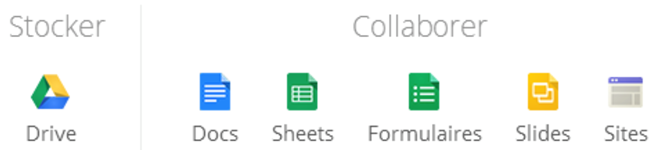
\includegraphics[scale=1]{images/googleDrive.png}
      \end{center}
      \caption{Exemple: la suite bureautique proposée par Google}
      \label{Google Cloud}
    \end{figure}

    \subsection{Le STAAT ou Storage As A Service (stockage en tant que service)}
    Le STAAT permet simplement des stocker nos données.

  \section{Le Cloud privé}
  Le Cloud privé est un Cloud propre à notre entreprise. A l’aide d’outils de virtualisation il est possible de transformer les serveurs existants au sein de l’entreprise. Cela créé un réseau puissant disponible, comme le Cloud public, à tout moment et à tout endroit mais géré entièrement par notre entreprise.

  \section{Las avantages du Cloud Computing}
  Les avantages du Cloud Computing sont nombreux. Si l’accessibilité est l’avantage le plus visible, il faut remarquer que l’utilisation du Cloud Computing permet à l’entreprise d’avoir une grande agilité, allant du démarrage rapide de son activité à un déploiement tout aussi rapide de nouvelles applications et donc un gain de temps et d’argent pour l’entreprise.\\

  De plus avec l’utilisation d’un Cloud public l’entreprise n’a plus d’investissement lourd en capital informatique, plus de dépendance en perte de temps et en entretient des infrastructures. Gains de places et de performances sont au rendez-vous.\\

  Cependant il faut soulever un petit bémol. En effet la contrepartie de tous cela est une dépendance totale envers internet et les prestataires de service. Ainsi qu’un coût croissant à mesure que les besoins de l’entreprises grandissent.

  \section{Quel Cloud choisir?}
  Si nous disposons déjà de serveurs et que nos besoins sont constants nous opterons pour le Cloud privé. Nous virtualiserons notre infrastructure et profiter de notre propre Cloud. Nos investissements sont ainsi préservés et nous gagnerions en productivité.\\

  En revanche, si nous ne disposons pas de serveurs ou que nous commençons tout juste notre activité et que nous ne souhaitons pas investir dans un parc informatique de serveur complet nous opterons pour un Cloud public. Economie et flexibilité sont au rendez-vous avec les services à la demande.\\

  Enfin si nous possédons des serveurs mais que notre activité fluctue beaucoup, nous demandant parfois des capacités plus fortes nous opterons pour le Cloud hybride. Nous concernerons ainsi notre autonomie avec notre Cloud privé et étendrons notre capacité ponctuellement avec le Cloud public.\\

  Pour conclure, si le Cloud Computing offre une grande disponibilité et une adaptabilité exemplaire, qui en font un service formidable, il n’en reste pas moins dépendant d’internet et les risques en matières de sécurité sont encore mal évalués.
